\section{Overview}
  \paragraph\
    In this chapter I describe about \emph{ntop}, Cassandra and the implementation of Cassandra plugin for \emph{ntop}. I also specify the design and implementation of Cassandra client for C that was developed using C-python API. 
% I have done few testing of my solution that I describe in results section.

\section{\emph{ntop}}
  \emph{ntop} is an open-source traffic measurement application written in C. \emph{ntop} design follows the UNIX philosophy: applications can be divided into small independent pieces that co-operate to achieve a common goal.
  \emph{ntop} has the following modules:
%AP: Case of the Missing Articles - I can write a nice long story about missing articles ``a, an, the'' in students' reports I think! Also, it seems not to matter how many times I talk about the singular and plural noun and verb combinations! I have to correct almost every sentence for this error. When will you guys ever learn?!
    \begin{enumerate}
     \item Packet Sniffer - Capture packets using \emph{libpcap} library and also from UNIX sockets.
     \item Packet Analyzer - Analyze packets captured by Packet Sniffer.
     \item Traffic Rules - \emph{ntop} allows traffic rules for capturing packets to filter out unnecessary packets.
     \item Report Engine - Report Engine displays analyzed output in an interactive web-based user interface. 
     \item Plugins - Using plugins anyone can extend \emph{ntop} to support extra features.
    \end{enumerate}

\subsection{Packet Sniffer}
\paragraph\
	Packet Sniffer captures packets using \emph{libpcap} library and stores them into internal buffer. This helps reduce packet drops	in a busty traffic environment. \emph{libpcap} is supported by all major Operating Systems, that allows \emph{ntop} to be portable to Windows and UNIX variants.

        \begin{figure}[htb]
          \centering
          \includegraphics[scale=.5]{ntoparc.jpg}
          \caption{Architecture of \emph{ntop}.} 
        \end{figure}

	\subsection{Packet Analyzer}
	 \paragraph\
	 Packet Analyzer gets packets from Packet Sniffer and processes those packets. Sniffed packets contains information about status of the network and that information is calculated by Packet Analyzer and then stored in 
	 RRD for future references.

	\subsection{Traffic Rules}
	\paragraph\
	  \emph{ntop} allows user to specify what kind traffic a user is interested in. Using \emph{libpcap} filter expression 
	  \emph{ntop} achieves this goal. Traffic Rules help \emph{ntop} to reduce some burden on memory as well CPU, make \emph{ntop} faster as it processes less number of packets.

	\subsection{Report Engine}
	\paragraph\
	  \emph{ntop} contains a web server by which users from any geological location can monitor their network.
	  Report Engine provides a beautiful user interface with time series graph drawn using RRDTool. Using Report Engine
	  a user can change the behavior of \emph{ntop} by changing its configuration parameters.

	\subsection{Plugins}
	 \paragraph\
	 \emph{ntop} has flexible design that allows user to add their own plugins. At startup \emph{ntop}
	 searches shared libraries (like .so, .dll files) to load  plugins. A plugin can access \emph{ntop}'s global 
	 data structure and can use API exported by \emph{ntop}.

\section{Cassandra Database}
\paragraph\
      Cassandra is a highly scalable and highly available database initially developed by Facebook using two famous approaches: GFS\cite{gfs} from Google and Dynamo\cite{dynamo} from Amazon. Cassandra is highly used in ebay and Netflix. 

      Cassandra's big data features are \cite{}
      \begin{enumerate}
       \item Elastic scalability.
       \item High availability.
       \item Distributed database design with no single point of failure.
       \item Blistering linear performance.
       \item Multiple datacenter based data distribution.
      \end{enumerate}

      \paragraph{Why Cassandra:} In one of our testbeds we are able to generate approximately 1000 NetFlow packets per second with only two nodes
      having 1 Gbps NIC card. The table below provides the amount of data generated by our testbed.\\
      \begin{tabular}{ccc}
      \\
      \hline
	  Packets generated& Time & Size of generated data \\
	  \hline
	  1000   & 1 second & 1.4MB\\
	  60 k   & 1 minute & 85 MB\\
	  3.6 m  & 1 hour    &  5 GB\\
      \end{tabular}\\

      It is clear that we cannot use RDMS based databases for storing flows in data center networks as they create explosive amount of data in a short time. 

      The features required of a database for flow monitoring are:
      \begin{enumerate}
       \item Scalability : so that huge amount of data can be stored according to the demand.
       \item High write throughput : As flow records are generated at a rapid pace in data center networks, a flow monitoring system needs to write them fast.
       \item Reasonable read performance : For real-time flow processing.
       \item MapReduce support: For offline flow processing it needs to support MapReduce to enable massive data crunching operation.
      \end{enumerate}

      \paragraph{Redis:} Redis is written in C. It has fast read-write performance but is not scalable. Redis cluster, which is expected to support scalability, is going to be launched by the end of 2013\cite{rrdcluster}. 
      \paragraph{HBase:} HBase is written in Java. It is scalable, has good read/write performance but is suitable only for batch processing. It has a single point of failure with Hadoop NameNode due to which HBase may lose data.
%for which HBase may lose data  .  

      \paragraph{Cassandra:} Cassandra meets all the requirements that are needed.
          \begin{figure}[htb]
	    \centering
	    \includegraphics[scale=.5]{cassathpt.png}
	    \caption{Cassandra Performance\cite{cassathpt}.} 
	  \end{figure}

\section{Cassandra C Client}
\paragraph\
      Cassandra C client is a wrapper developed by me around Cassandra Python client, $Pycassa$. This allows any user to call Cassandra API from a C program.
%I used C-Python API to write wrapper around Python's Pycassa API. 
Pycassa uses Thrift RPC call to communicate with Cassandra. Fig. \ref{cass-c-api} shows the architecture of the Cassandra C API.
      
%Figure 2.3 describes how a C client API call finally reach Cassandra. 
Cassandra C client API has three major classes of APIs. These are 
      \begin{enumerate}
       \item Schema Manipulation API: Manages schema definitions of Cassandra.
       \item Data Manipulation API: Inserts or retrieves data from Cassandra. 
       \item Utility API:  API that do some common useful work. 
      \end{enumerate}

      \begin{figure}[htb]
	 \centering
         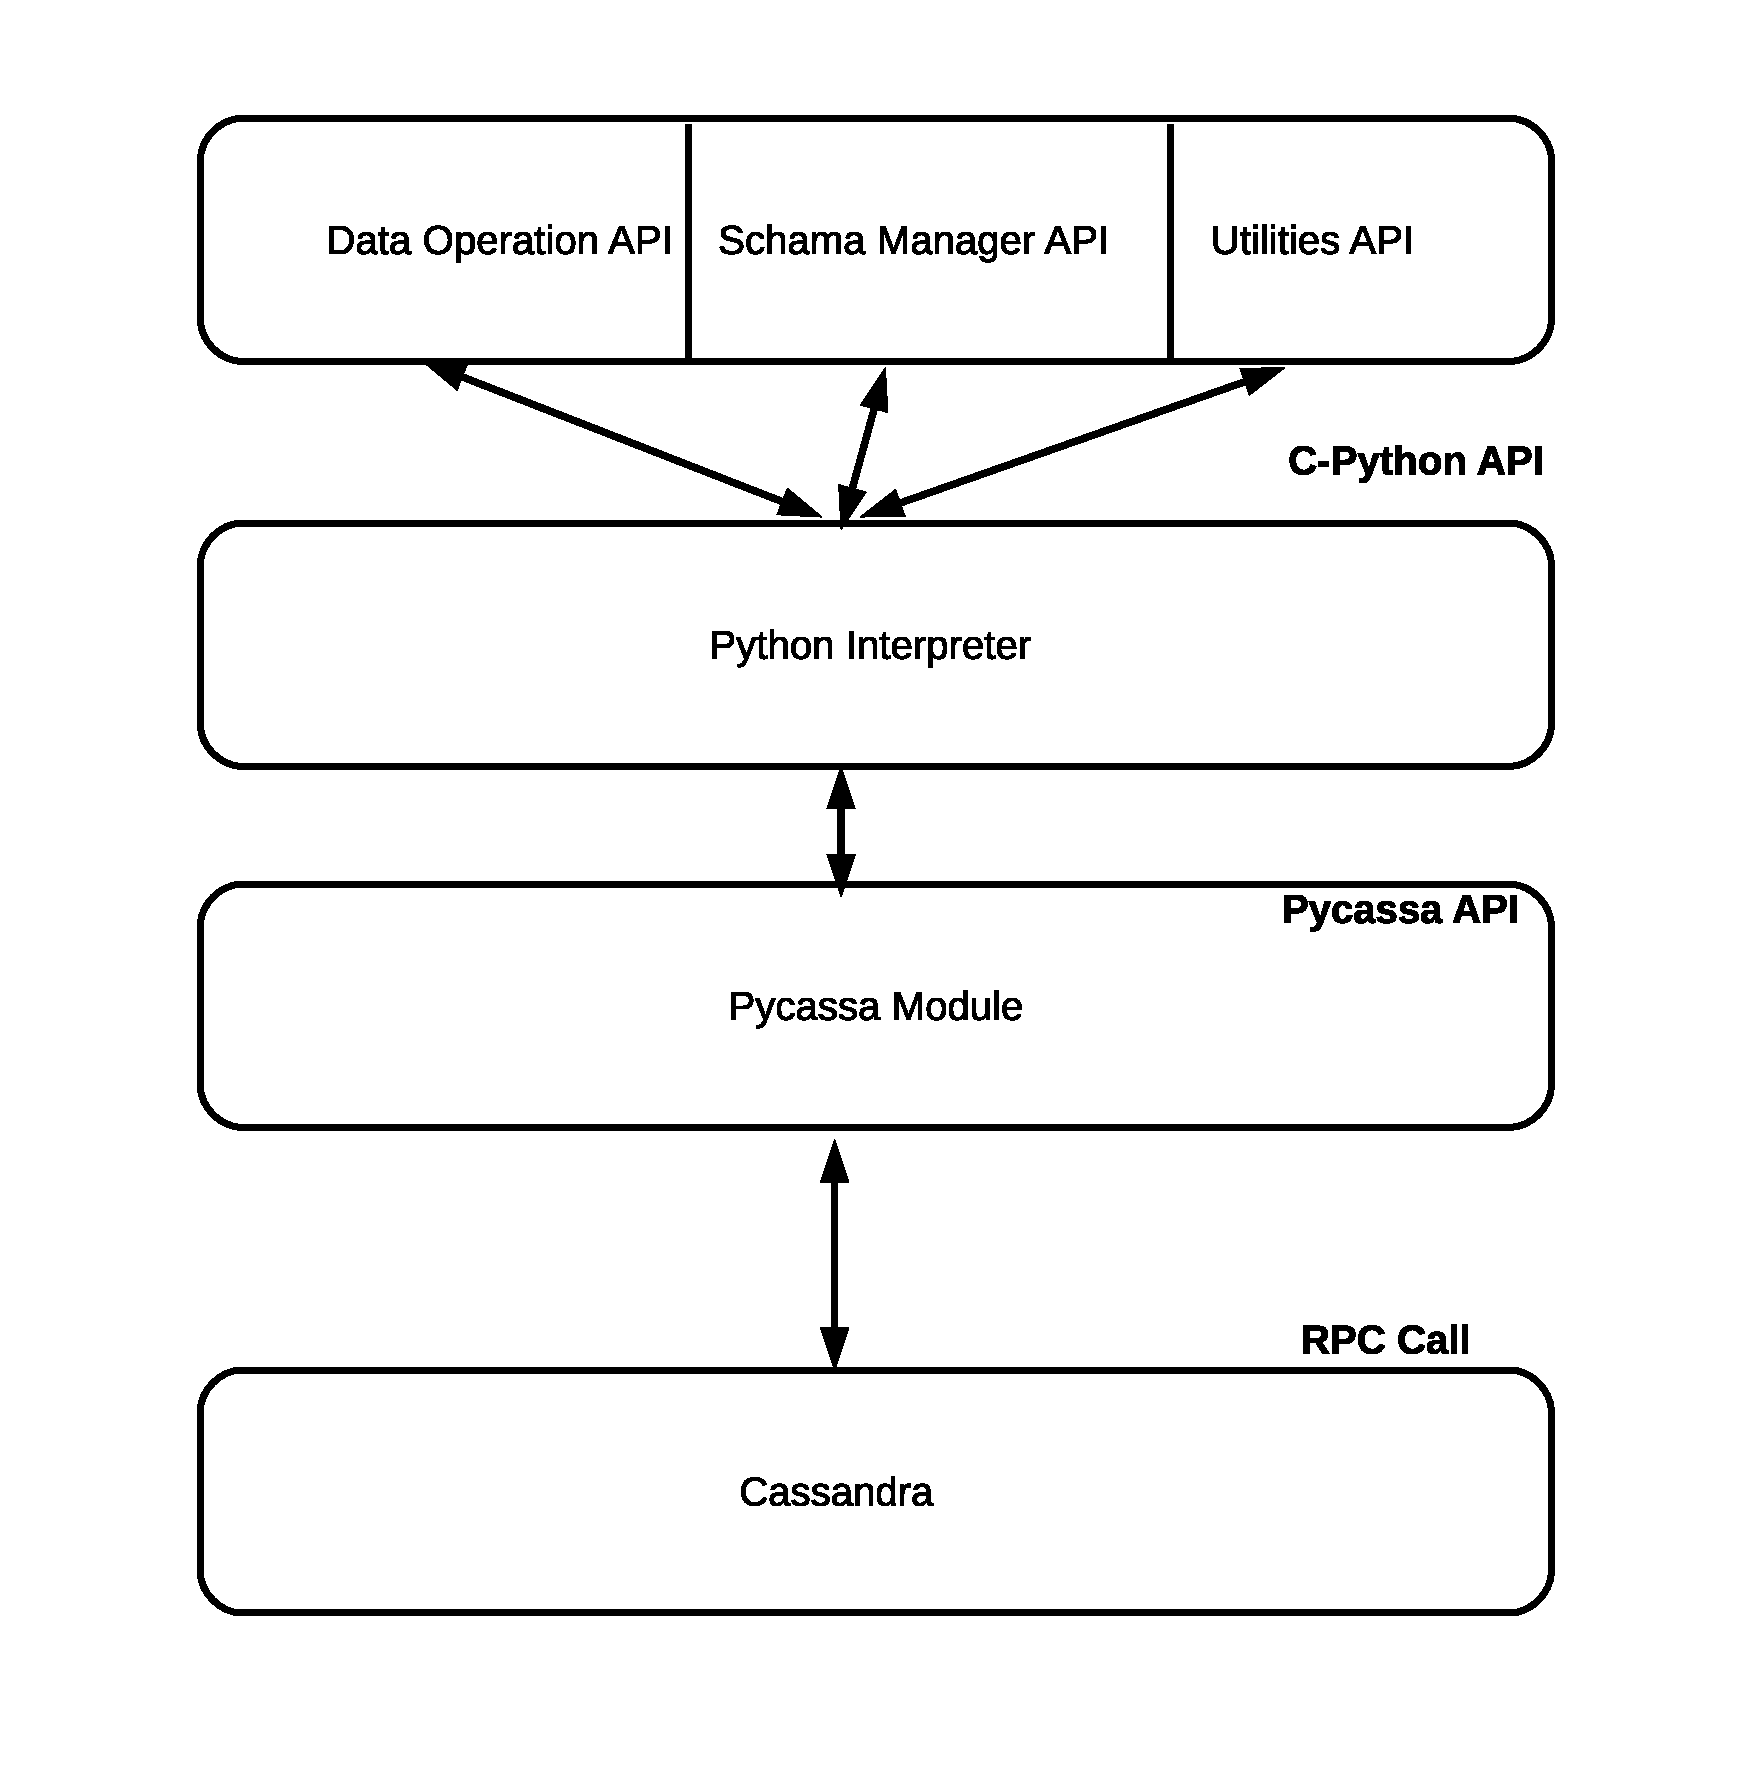
\includegraphics[scale=0.3]{C_client.eps}
         \caption{API interaction with Cassandra }
	\label{cass-c-api}
      \end{figure}

\subsection{Schema Manipulation API}
      \paragraph\
      These APIs allow one to create or delete keyspace and column families. 

      \begin{enumerate}
       \item {\bf cassandraCreateKeyspace}(name, server, rf, strategy): Create a keyspace on the server with the given replication factor(rf) and strategy.
	    Supported strategies are :
	     \begin{enumerate}
	      \item SimpleStrategy : Replication strategy that simply chooses consecutive nodes in the ring for replicas.
	      \item NetworkTopologyStrategy : Replication strategy that puts a number of replicas in each data center.
	      \item OldNetworkTopologyStrategy : Same as NetworkTopologyStrategy with few limitations that solved in NetworkTopologyStrategy. %AP re-write this.
	     \end{enumerate}

       \item {\bf cassandraCreateColumnFamily}(name, keyspace, comparator, server): Create a column family on the keyspace with the given comparator. 
	      Supported comparators are :
		    \begin{enumerate}
		     \item AsciiType
		     \item DoubleType
		     \item IntegerType
		     \item BytesType
		     \item LongType
		     \item FloatType
		     \item TimeUUIDType
		    \end{enumerate}

      \item {\bf cassandraDropColumnFamily}(name, keyspace, server): Delete the given column family, $name$, from the keyspace.

      \item {\bf cassandraDropKeyspace}(name, server): Delete keyspace from the server.
      \end{enumerate}

    \subsection{Data Manipulation API}
    \paragraph\
    These APIs deal with insertion and retrieval of data from the Cassandra server.

      \begin{enumerate}
       \item {\bf cassandraConnect}(keyspace, columnfamily, server): Create a connection and store the connection object in the internal Python dictionary for later use. As connection creation takes time, connection objects are cached in the Python dictionary.

       \item {\bf cassandraInsert}(id, key, value, column name): Insert a key-value pair in the column family referred by $id$.

       \item {\bf cassandraGet}(id, key): Return a dictionary of key-value pairs from  the column family referred by $id$.

       \item {\bf cassandraGetItem}(dictionary, position, name, value): Return a column name and value from the dictionary specified by position.  %AP: rewrite
      \end{enumerate}

    \subsection{Utility API}
    \paragraph\
    These APIs provide general functionality that we need.

      \begin{enumerate}
       \item {\bf isExistPycassa}(): Check existence of pycassa on the system.
       \item {\bf isExistKeyspace}(name, server): Check existence of keyspace on the server.
       \item {\bf isExistColumnfamily}(name, keyspace, server): Check existence of columnfamily on the keyspace. 
      \end{enumerate}

      \section{Cassandra Plugin for \emph{ntop}}
      Cassandra Plugin is developed in C as a shared object. \emph{ntop} uses  shared objects principles to provide plugins, 
      that allows dynamic linking of compiled shared objects  to \emph{ntop} to add extra features.

      \textbf{The APIs supported by \emph{ntop} for plugin support are given below:}\\
     
     \begin{tabular}{|l|l|}
	\hline
	\textbf{API name} &  \textbf{Details}\\
	\hline
	int(*IntFunct)(void); & Called at initialization of the plugin.\\
	\hline
	void(*VoidFunct)(u\_char); & Called at termination of the plugin.\\
	\hline
	void(*PluginHTTPFunct)(char* url); & HTTP request handler function.\\
	\hline
      \end{tabular}
      
      
      \paragraph{API of Cassandra Plugin:} Given below are the APIs developed by me for a
      Cassandra Plugin for \emph{ntop}.\\
      
      \begin{enumerate}
       \item {\bf initCassandraFunct } (void): Initialize Cassandra Plugin. It checks for pycassa module, availability of the Cassandra server and then invokes cassandraMainLoop.
       \item {\bf termCassandraFunct} (u\_char termNtop): Terminates Cassandra Plugin.
       \item {\bf handlecassandraHTTPrequest} (char *\_url): It gets a web request from the web browser and serves them.\\
       \item {\bf cassandraMainLoop}(void) : This API does all major work described below:
	      \begin{enumerate}
	      \item Reads configuration files and initializes the data structure needed to store data.
	       \item Identifies sniffed interface, gets statistics from global variables and stores into Cassandra.
	       \item Identifies NetFlow socket, gets data from global variables and stores them to Cassandra. 
	      \end{enumerate}
      \end{enumerate}

      \subsection{Architecture}
      Figure 2.4 shows the architecture for Cassandra Plugin .
            \begin{figure}[htb]
	    \centering
	    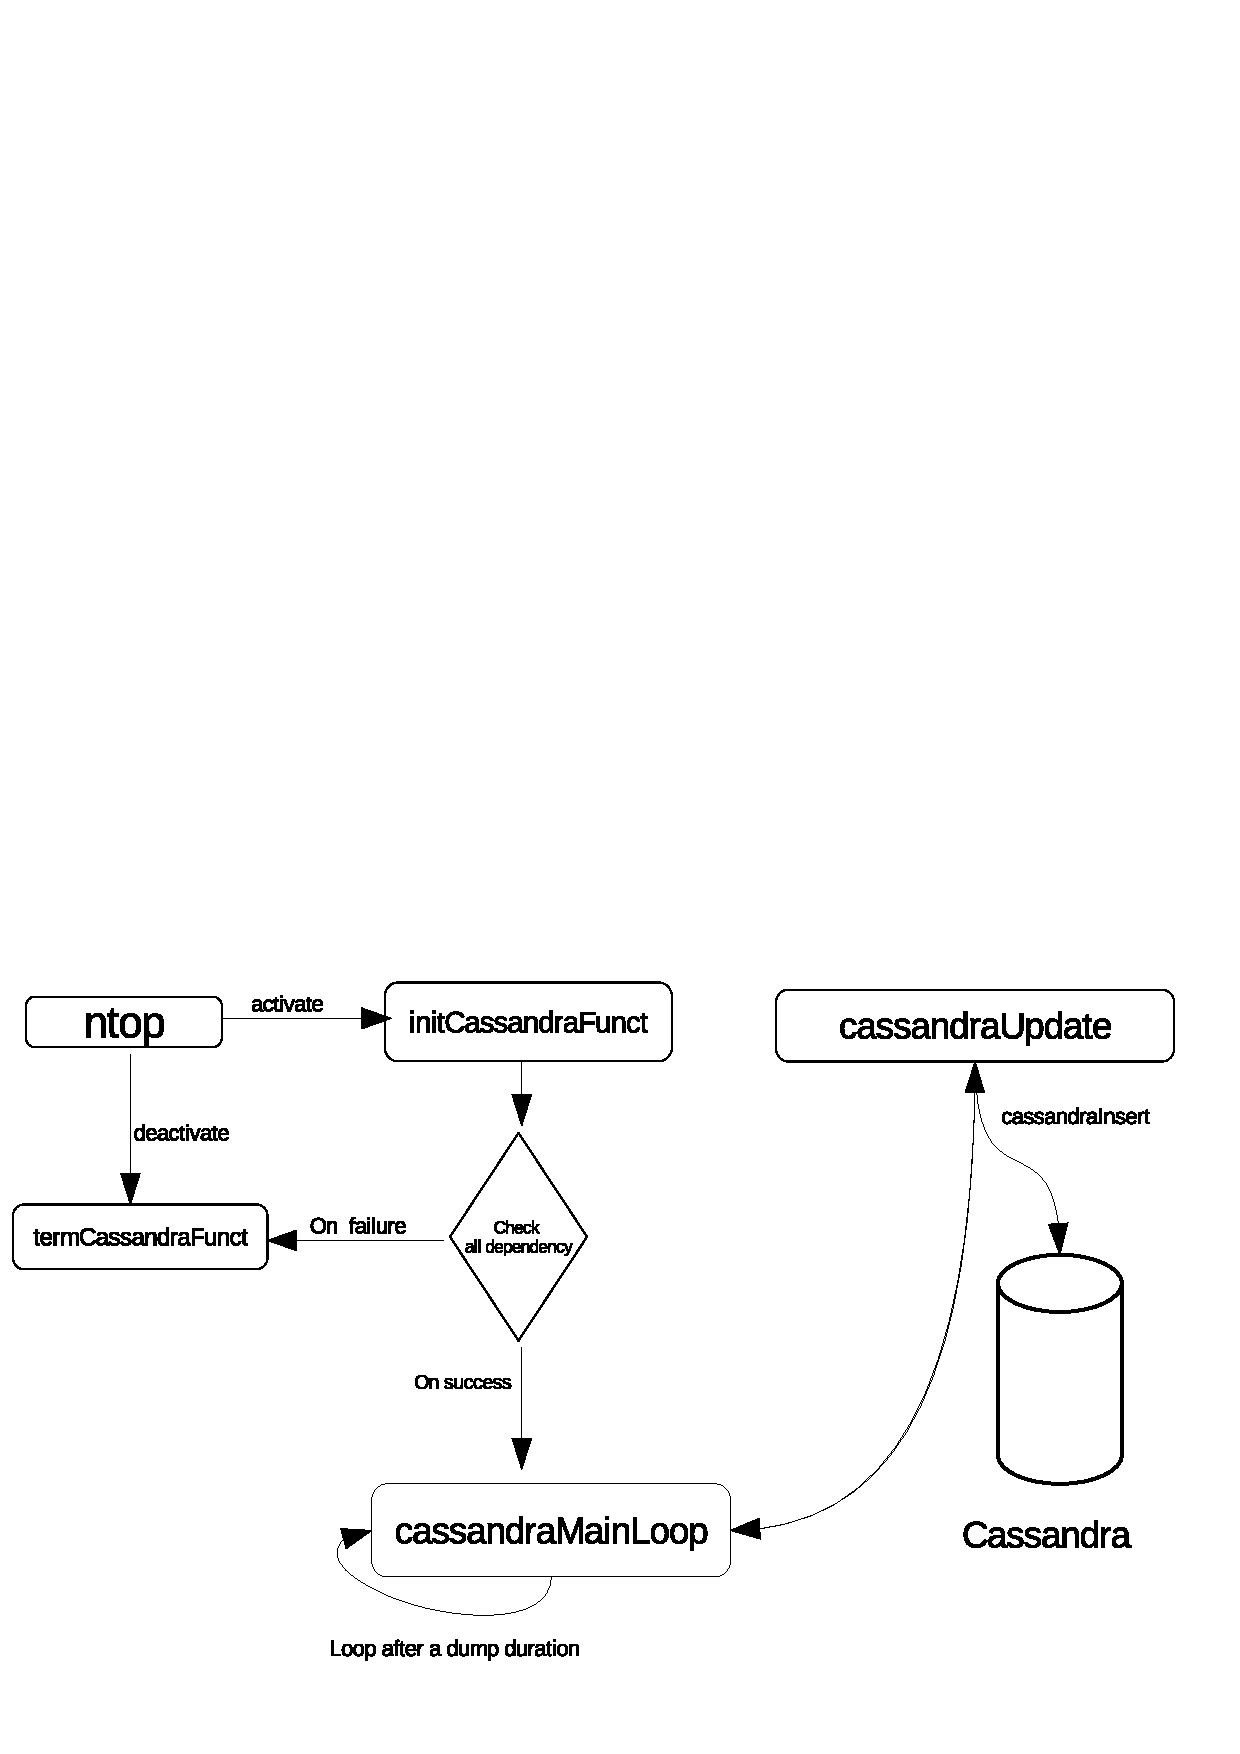
\includegraphics[scale = .5]{lfc.pdf}
	    \caption{Architecture of Cassandra Plugin.} 
	  \end{figure}
